\normalfalse \difficiletrue \tdifficilefalse
\correctionfalse

%\UPSTIidClasse{12} % 11 sup, 12 spé
%\newcommand{\UPSTIidClasse}{12}

\exer{Mouvement RT -- RSG  $\star\star$ \label{C2:08:08}}
\setcounter{numques}{0}
\UPSTIcompetence[2]{C2-08}
\UPSTIcompetence[2]{C2-09}
\index{Compétence C2-08}
\index{Compétence C2-09}
\index{Torseur cinétique}
\index{Torseur dynamique}
\index{Mécanisme à 1 rotations, 1 translation et RSG}
\ifcorrection
\else
\textbf{Pas de corrigé pour cet exercice.}
\fi

\ifprof
\else
Soit le mécanisme suivant. On a $\vect{IA}=R\vect{j_0}$ et $\vect{AB}=\lambda(t)\vect{i_1}$. De plus $R=\SI{15}{mm}$.
On fait l'hypothèse de roulement sans glissement au point $I$. De plus :
\begin{itemize}
\item $G_1$ désigne le centre d'inertie de \textbf{1} tel que $\vect{AG_1}=-\ell\vect{i_1}$, on note $m_1$ la masse de \textbf{1} et $\inertie{G_1}{1}=\matinertie{A_1}{B_1}{C_1}{0}{0}{0}{\bas{1}}$; 
\item $G_2=B$ désigne le centre d'inertie de \textbf{2}, on note $m_2$ la masse de \textbf{2} et $\inertie{G_2}{2}=\matinertie{A_2}{B_2}{C_2}{0}{0}{0}{\bas{2}}$.
\end{itemize}
\begin{center}
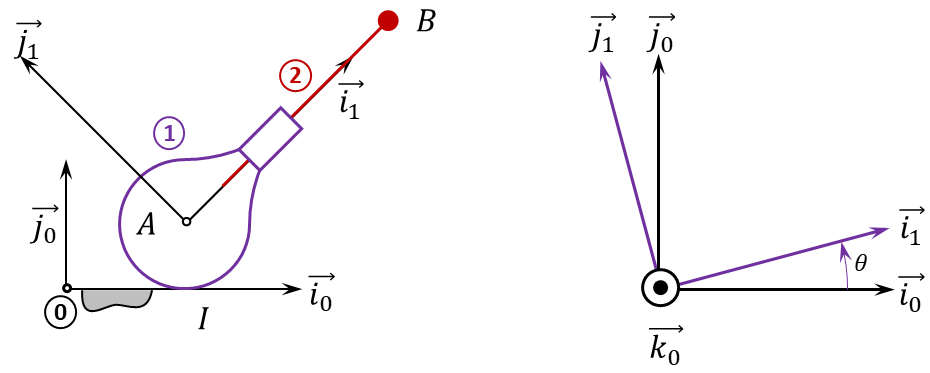
\includegraphics[width=\linewidth]{09_RT_RSG_01}
\end{center}

On donne  $\vectv{B}{2}{0} = \lambdap\vi{1} + \thetap\left(\lambda(t)\vj{1}-R\vi{0} \right)$
et

$\vectg{B}{2}{0}  = \lambdapp(t)\vi{1} %+\lambdap(t)\thetap\vj{1} 
+ \thetapp(t)\left(\lambda(t)\vj{1}-R\vi{0} \right)
+ \thetap(t)\left(2\lambdap(t)\vj{1}-\lambda(t)\thetap\vi{1} \right)
$.


\fi



\question{Déterminer $\vectrd{2}{0}\cdot \vect{i_1}$}
\ifprof

Par définition, $\vectrd{2}{0} =  m_2 \vectg{G_2}{2}{0}=  m_2 \vectg{B}{2}{0}$.

\vspace{.5cm}

\textbf{Calcul de $ \vectv{B}{2}{0}$ :}

$\vectv{B}{2}{0}=\vectv{B}{2}{1}+\vectv{B}{1}{0}$.

D'une part,  $\vectv{B}{2}{1}=\lambdap\vi{1}$.

D'autre part, en utilisant le roulement sans glissement en $I$, 
$\babarv{B}{I}{1}{0} $ $=\vect{0}+\left(-\lambda(t)\vi{1}-R\vj{0} \right)\wedge\thetap \vk{0}$
$=-\thetap\left(\lambda(t)\vi{1}\wedge \vk{0}+R\vj{0}\wedge \vk{0} \right)$
$=\thetap\left(\lambda(t)\vj{1}-R\vi{0} \right)$.

Au final, $\vectv{B}{2}{0} = \lambdap\vi{1} + \thetap\left(\lambda(t)\vj{1}-R\vi{0} \right)$.

\vspace{.5cm}

\textbf{Calcul de $ \vectg{B}{2}{0}$ :}

$\vectg{B}{2}{0} = \deriv{\vectv{B}{2}{0}}{\rep{0}}$
$ = \lambdapp(t)\vi{1} +\lambdap(t)\thetap\vj{1} 
+ \thetapp(t)\left(\lambda(t)\vj{1}-R\vi{0} \right)
+ \thetap(t)\left(\lambdap(t)\vj{1}-\lambda(t)\thetap\vi{1} \right)
$.

\else
\fi

\question{Déterminer $\vectmd{I}{1+2}{0}\cdot \vect{k_0}$}
\ifprof
\else
\fi


\ifprof
\else
\begin{flushright}
\footnotesize{Corrigé  voir \ref{C2:08:08}.}
\end{flushright}%
\fi